\documentclass[a4paper, 10pt]{article}
\usepackage[utf8]{inputenc}
\usepackage[spanish]{babel}
\usepackage{hyperref}
\usepackage{tabularx}
\usepackage{inconsolata}
\usepackage{enumitem}
\usepackage{graphicx}
\usepackage{subfigure}
\usepackage{listings}
\usepackage{color}
\usepackage{appendix}
\usepackage{mdframed}

\definecolor{mygreen}{rgb}{0,0.6,0}
\definecolor{mygray}{rgb}{0.5,0.5,0.5}
\definecolor{mymauve}{rgb}{0.58,0,0.82}

\lstset{ %
	backgroundcolor=\color{white},   % choose the background color; you must add \usepackage{color} or \usepackage{xcolor}
	basicstyle=\footnotesize,        % the size of the fonts that are used for the code
	breakatwhitespace=false,         % sets if automatic breaks should only happen at whitespace
	breaklines=true,                 % sets automatic line breaking
	captionpos=b,                    % sets the caption-position to bottom
	commentstyle=\color{mygreen},    % comment style
	deletekeywords={...},            % if you want to delete keywords from the given language
	escapeinside={\%*}{*)},          % if you want to add LaTeX within your code
	extendedchars=true,              % lets you use non-ASCII characters; for 8-bits encodings only, does not work with UTF-8
	frame=single,                    % adds a frame around the code
	keepspaces=true,                 % keeps spaces in text, useful for keeping indentation of code (possibly needs columns=flexible)
	keywordstyle=\color{blue},       % keyword style
	language=Octave,                 % the language of the code
	morekeywords={*,...},            % if you want to add more keywords to the set
	numbers=left,                    % where to put the line-numbers; possible values are (none, left, right)
	numbersep=5pt,                   % how far the line-numbers are from the code
	numberstyle=\tiny\color{mygray}, % the style that is used for the line-numbers
	rulecolor=\color{black},         % if not set, the frame-color may be changed on line-breaks within not-black text (e.g. comments (green here))
	showspaces=false,                % show spaces everywhere adding particular underscores; it overrides 'showstringspaces'
	showstringspaces=false,          % underline spaces within strings only
	showtabs=false,                  % show tabs within strings adding particular underscores
	stepnumber=2,                    % the step between two line-numbers. If it's 1, each line will be numbered
	stringstyle=\color{mymauve},     % string literal style
	tabsize=2,                       % sets default tabsize to 2 spaces
	title=\lstname                   % show the filename of files included with \lstinputlisting; also try caption instead of title
}

\makeatletter
\def\@seccntformat#1{%
  \expandafter\ifx\csname c@#1\endcsname\c@section\else
  \csname the#1\endcsname\quad
  \fi}
\makeatother

\newcommand{\tabitem}{\vspace{1mm}~~\llap{\textbullet}~~}

\hypersetup{
    colorlinks=true,
    citecolor=black,
    linkcolor=black,
    urlcolor=blue
}

%% Titulo y autores
\title{Sistemas Informáticos 2\\Práctica 3}
\author{Cristina Kasner Tourné\and Guillermo Guridi Mateos}
\date{\today}

%% Documento
\begin{document}
\maketitle
\newpage

\section{Ejercicio 1}
\begin{mdframed}
	Preparar 3 máquinas virtuales con acceso SSH entre ellas. Esta tarea es necesaria para la
	correcta gestión del cluster que definiremos en el próximo apartado. Las VMs las denominaremos
	\begin{itemize}
		\item si2srv01: Dirección IP 10.X.Y.1, 768MB RAM
		\item si2srv02: Dirección IP 10.X.Y.2, 512MB RAM
		\item si2srv03: Dirección IP 10.X.Y.3, 512MB RAM 
	\end{itemize}
	
	RECUERDE RANDOMIZAR LAS DIRECCIONES MAC DE CADA COPIA, Y ELIMINAR EL FICHERO 
	
	/etc/udev/rules.d/70-persistent-net.rules 
	
	ANTES DE INTENTAR USAR EL NODO.
	
	
	En la primera máquina (10.X.Y.1), generaremos el par de claves con DSA. A continuación importaremos la
	clave pública en cada uno de los otros dos nodos (10.X.Y.2 y 10.X.Y.3). Probaremos a acceder por SSH
	desde .1 a .2 y .3, comprobando que no requiere la introducción de la clave. Obtener una evidencia del
	inicio remoto de sesión mediante la salida detallada (ssh –v si2@10.X.Y.2 y ssh –v si2@10.X.Y.3 ). Anote
	dicha salida en la memoria de prácticas.
	
	
	Una vez realizado este punto, detendremos las tres máquinas virtuales y obtendremos una copia de
	las mismas a algún medio externo (USB) para los consiguientes apartados de esta práctica.
	También es recomendable que preserve los directorios .ssh de cada uno de los nodos
\end{mdframed}




Hemos realizado el ejercicio siguiendo los pasos que nos daban en el enunciado y no hemos tenido ningún problema.
\newpage
\section{Ejercicio2}


\begin{mdframed}
	 Realizar los pasos del apartado 4 con el fin de obtener una configuración válida del cluster
	 \texttt{SI2Cluster}, con la topología indicada de 1 DAS y 2 nodos SSH de instancias. Inicie el cluster. 
	 
	 Liste las instancias del cluster y verifique que los pids de los procesos Java (JVM) correspondientes están
	 efectivamente corriendo en cada una de las dos máquinas virtuales. Adjunte evidencias a la memoria de la
	 práctica. 
\end{mdframed}	

	Adjuntamos la imagen con  el resultado de ejecutar el comando \texttt{asadmin --user admin --passwordfile /opt/SI2/passwordfile list-instances –l}
 
 	Aquí se pueden observar los pids de cada una de las instancias.
 	\begin{figure}[hbtp]
 		\centering
 		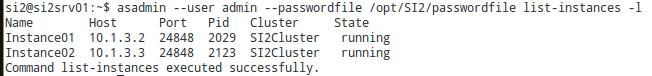
\includegraphics[width=0.8\textwidth]{../../P3/pantallazos/ej2_listar_instancias.png}
 		\caption {Lista de instancias}
 	\end{figure}
 \newpage
 \section{Ejercicio3}
 
 \begin{mdframed}
 	 Pruebe a realizar un pago individualmente en cada instancia. Para ello, identifique los
 	 puertos en los que están siendo ejecutados cada una de las dos instancias (IPs 10.X.Y.2 y 10.X.Y.3
 	 respectivamente). Puede realizar esa comprobación directamente desde la consola de administración,
 	 opción Applications, acción Launch, observando los Web Application Links generados.
 	 
 	 Realice un único pago en cada nodo. Verifique que el pago se ha anotado correctamente el nombre de la
 	 instancia y la dirección IP. Anote sus observaciones (puertos de cada instancia) y evidencias (captura de
 	 pantalla de la tabla de pagos). 
 \end{mdframed}
 
Este ejercicio nos ha costado un poc más que los anteriores ya que hemos tenido un par de fallos trabajando con la base de datos.

Finalmente hemos conseguido solucionarlos y realizar los pagos.

Para encontrar el puerto de cada instancia hemos mirado en la consola de administración, tal y como nos decía el enenuciado. Los puertos son:
\begin{itemize}
	\item Instancia01 $\rightarrow$ 28080
	\item Instancia02 $\rightarrow$ 28080
\end{itemize}

Adjuntamos las pantallas que confirma la realización de pago con cada una de las instancias y la base de datos resultante.

\begin{figure}[htbp]
	\centering
	\subfigure[Instancia01]{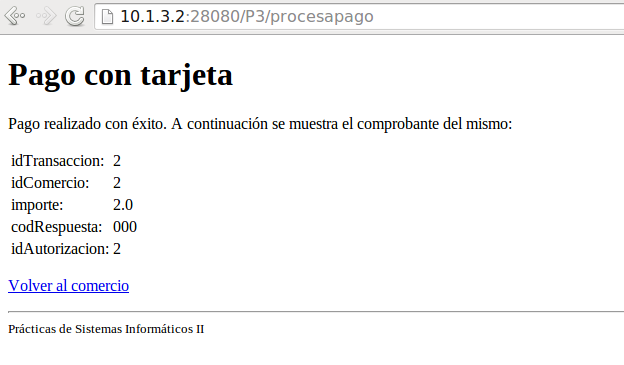
\includegraphics[width=40mm]{../../P3/pantallazos/ej3_instancia1.png}}
	\subfigure[Instancia02]{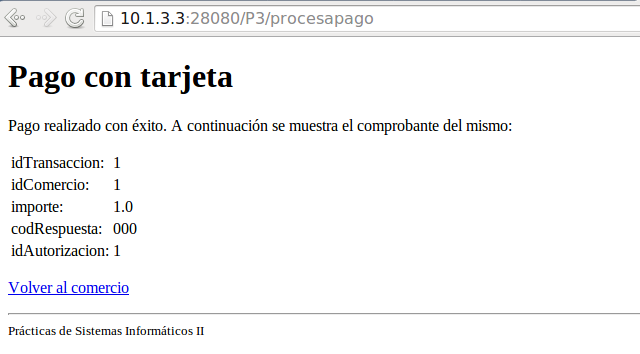
\includegraphics[width=40mm]{../../P3/pantallazos/ej3_instancia2.png}}
		\subfigure[Base de datos]{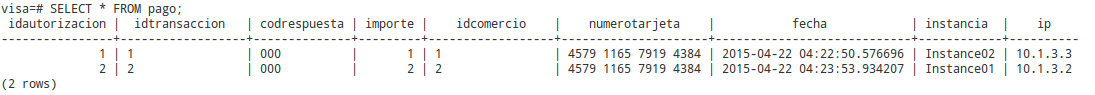
\includegraphics[width=70mm]{../../P3/pantallazos/ej3_bd.png}}
	\caption{Pago instancias}
\end{figure}
\newpage
\section{Ejercicio4}

\begin{mdframed}
	Probar la influencia de jvmRoute en la afinidad de sesión. 
	\begin{enumerate}
		\item Eliminar todas las cookies del nevegador 
		\item Sin la propiedad jvmRoute, acceder a la aplicación P3 a través de la URL del balanceador:
		\texttt{http://10.X.Y.1/P3}
		\item Completar el pago con datos de tarjeta correctos. 
		\item Repetir los pagos hasta que uno falle debido a la falta de afinidad de sesión. 
		\item  Mostrar la cookie “JSESSIONID” correspondiente a la URL del balanceador donde se vea: 
		
		\texttt{Name: JSESSIONID}
			
		\texttt{Content: YYYYYYYYYYYYYYYYYYY}
			
		\texttt{Domain: 10.X.Y.1}
			
		\texttt{Path: /P3 }
		
		\item Añadir la propiedad “jvmRoute” al cluster y rearrancar el cluster. 
		\item Eliminar todas las cookies del nevegador. 
		\item Acceso a la aplicación P3 a través de la URL del balanceador: 
		
		\texttt{http://10.X.Y.1/P3}
		\item  Completar el pago con datos de tarjeta correctos. Se pueden repetir los pagos y no fallarán. 
		\item  Mostrar la cookie “JSESSIONID” correspondiente a la URL del balanceador donde se vea:
		
		\texttt{Name: JSESSIONID}
		
		\texttt{Content: ZZZZZZZZZZZZZZZZZZZZZZ}
		
		\texttt{Domain: 10.X.Y.1}
		
		\texttt{Path: /P3} 
		
		Mostrar las pantallas y comentar: las diferencias en el contenido de las cookie respecto a jvmRoute, cómo esta diferencia afecta a la afinidad y por qué.
	\end{enumerate}
\end{mdframed}
\newpage
Configuramos el balanceador de carga y comprobamos que todo se ha hecho correctamente:

\begin{figure}[hbtp]
	\centering
	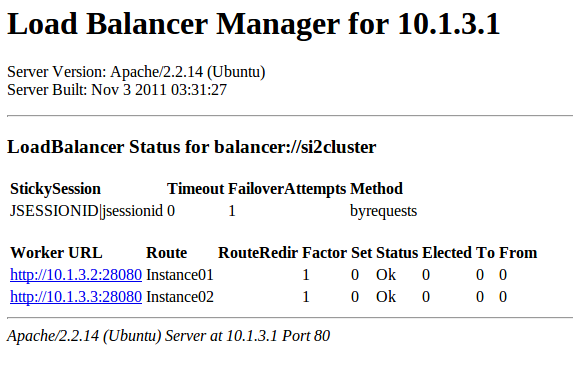
\includegraphics[width=0.8\textwidth]{../../P3/pantallazos/manager.png}
	\caption { Página de status del balanceador }
\end{figure}


Una vez hecho esto realizamos las actividades del ejercicio 4:

- Borramos las cookies:
\begin{figure}[hbtp]
	\centering
	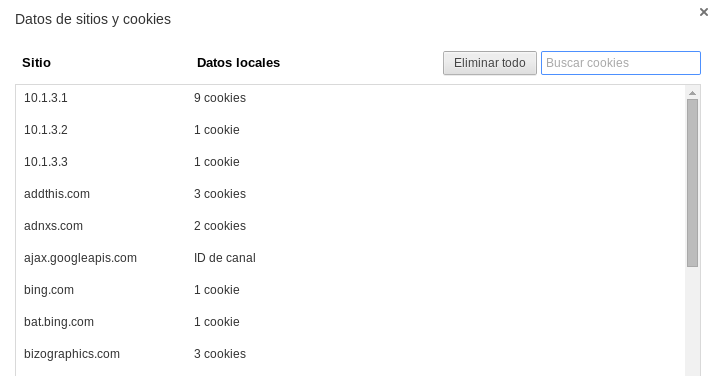
\includegraphics[width=0.8\textwidth]{../../P3/pantallazos/ej4_cookies.png}
	\caption { Cookies }
\end{figure}

\newpage
\section{Ejercicio5}
\begin{mdframed}
	 Probar el balanceo de carga y la afinidad de sesión, realizando un pago directamente contra la dirección del cluster
	 \texttt{ http://10.X.Y.1/P3 }
	 desde distintos ordenadores. Comprobar que las peticiones se reparten entre ambos nodos del cluster, y
	 que se mantiene la sesión iniciada por cada usuario sobre el mismo nodo. 
\end{mdframed}

\section{Ejerecicio6}
\begin{mdframed}
	\textbf{Comprobación del proceso de fail-over.} Parar la instancia del cluster que haya tenido
	menos elecciones hasta el momento. Para ello, identificaremos el \textbf{pid} (identificador del proceso java) de la
	instancia usando las herramientas descritas en esta práctica o el mandato ‘ps –aef | grep java’.
	Realizaremos un \textbf{kill -9 pid} en el nodo correspondiente. Vuelva a realizar peticiones y compruebe
	(accediendo a la página /balancer-manager) que el anterior nodo ha sido marcado como “erróneo” y que
	todas las peticiones se dirijan al nuevo servidor. Adjunte la secuencia de comandos y evidencias obtenidas
	en la memoria de la práctica. 
\end{mdframed}

\section{Ejercicio7}
\begin{mdframed}
	 \textbf{Comprobación del proceso de fail-back.} Inicie manualmente la instancia detenida en el
	 comando anterior. Verificar la activación de la instancia en el gestor del balanceador. Incluir todas las
	 evidencias en la memoria de prácticas. \textbf{Consulte los apéndices para información detallada de
	 comandos de gestión individual de las instancias.}
\end{mdframed}

\section{Ejercicio8}
\begin{mdframed}
	 \textbf{Fallo en el transcurso de una sesión.}
	 \begin{itemize}
	  \item Desde un navegador, comenzar una petición de pago introduciendo los valores del mismo en la
	  pantalla inicial y realizando la llamada al servlet ComienzaPago.
	  \item Al presentarse la pantalla de "Pago con tarjeta", leer la instancia del servidor que ha procesado la
	  petición y detenerla. Se puede encontrar la instancia que ha procesado la petición revisando la
	  cookie de sesión (tiene la instancia como sufijo), el balancer-manager o el server.log de cada
	  instancia.
	  \item Completar los datos de la tarjeta de modo que el pago fuera válido, y enviar la petición.
	  \item Observar la instancia del cluster que procesa el pago, y razonar las causas por las que se rechaza
	  la petición. 	
	 \end{itemize}
	
\end{mdframed}

\section{Ejercicio9}
\begin{mdframed}
	Modificar el script de pruebas JMeter desarrollado durante la P2. (P2.xml) Habilitar un ciclo de
	1000 pruebas en un solo hilo contra la IP del cluster y nueva URL de la aplicación:
	\texttt{http://10.X.Y.1/P3}
	Eliminar posibles pagos previos al ciclo de pruebas. Verificar el porcentaje de pagos realizados por cada
	instancia, así como (posibles) pagos correctos e incorrectos. ¿qué algoritmo de reparto parece haber
	seguido el balanceador? Comente todas sus conclusiones en la memoria de prácticas. 
\end{mdframed}

\newpage
\appendix
\section{Apéncices}

\end{document}